\section{VDMS Design \& Implementation}
\label{arch}

In this section, we briefly describe VDMS design principles and implementation,
(most of it is already cover in previous work \cite{vdms-nips}).
Figure \ref{fig:arch} depicts the high-level architecture of VDMS.
VDMS implements a client-server architecture that handles client
requests concurrently and coordinates query execution across
the metadata and data components in order to return a unified response.

The metadata component is the \textit{Persistent Memory Graph
Database} (PMGD). The (visual) data component is our Visual Compute Module.
The Visual Compute Module enables machine friendly enhancements to
visual data, exposing high-level abstractions to the \textit{Request Server} for
dealing with a variety of images and video formats (through OpenCV),
and different methods for indexing for Feature Vectors
(including Facebook's Faiss \cite{faiss}, TileDB \cite{TileDB}).
VDMS and its components are fully available open source
\footnote{https://github.com/IntelLabs/\{vdms, pmgd\}}.
We briefly describe each of the main components as follows:

\begin{figure}[]
\centering
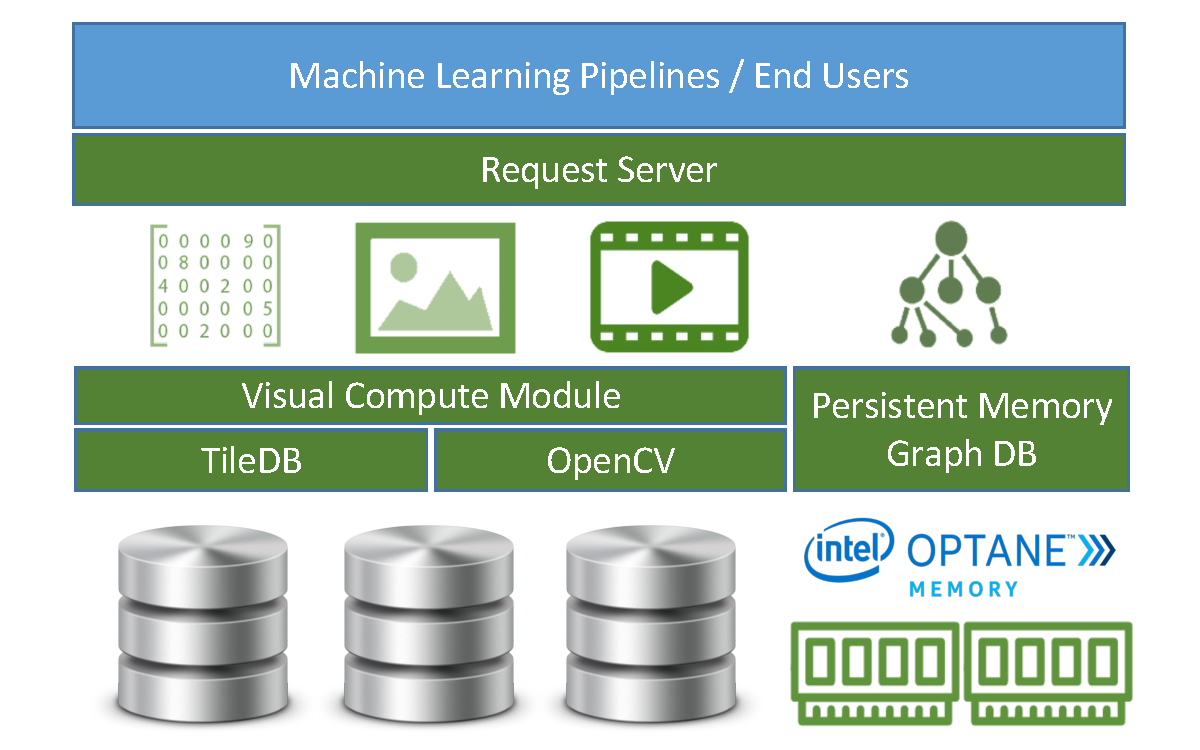
\includegraphics[width=1\columnwidth]{figures/vdms_arch.pdf}
\caption{VDMS Architecture}
\label{fig:arch}
\end{figure}

\textbf{Persistent Memory Graph Database:}
We use PMGD to provide an efficient storage
solution addressing the increasing popularity of connected data and
applications that benefit from graph like processing, we have designed
and implemented an in-persistent-memory graph database, PMGD, optimized
to run on a platform equipped with persistent memory.
PMGD provides a property graph model of data storage with the traditional
atomicity, consistency, isolation, and durability properties expected from
databases. The graph model makes it very suitable for the data model and
access patterns shown by visual metadata.
With its natural ability to extend the schema very
easily (due to the use of a property graph model),
we can support new developments in machine learning that can lead to
enhancements to existing metadata over time.
The specific details on how the data structures are optimized for persistent
memory, and the performance comparison with other graph databases is on-going
work that will be publish separately.
PMGD has been design and optimized for persistent memory technologies
like 3D XPoint~\cite{IntelXPoint15}, which
promise storage providing nearly the speed of DRAM and the
durability of block-oriented storage.

\textbf{Visual Compute Module:} This module was designed to provide
an abstraction layer for interacting with with visual data.
For traditional formats (jpg, png, tiff, mp4, etc),
the interface is an abstraction layer over OpenCV. However, it also provides a
way to use novel formats that are better suited for visual analytics: a novel,
array-based lossless image format. This format is built on the array data
manager TileDB~\cite{TileDB} and is well suited for images that are used in
visual analytics.
This module also provides support for videos, enabling operations like
encoding/decoding/transcoding and resize as part of VDMS interface.
Feature vector support is provided through an implementation based
on high-dimensional sparse arrays, also using TileDB, which contains both
storage and search functionality over feature vectors.
In addition, the VCL provides a wrapper
for another high-dimensional index implementation,
Facebook's Faiss~\cite{faiss}.

\textbf{Request Server:}
Developers and users of machine learning frameworks and data science
applications favor simpler interfaces to access and process data and cannot
be expected to deal with two different ways of interacting with information
(metadata and visual data) instead of focusing on the
algorithmic parts of their pipelines.
VDMS takes care of coordinating client requests across the metadata and the
data as well as efficiently manages multiple clients through its Request
Server component, by implementing a JSON-based API.
It decomposes the command into
metadata and data requests, invokes the relevant calls behind the scene,
and returns a coherent response to the user after applying any additional
operations (explained in the next section).

\textbf{Client Library:}
A user application can use the VDMS API by defining metadata conforming to the
query protocol we have defined.
The client side VDMS library provides a simple query function that
accepts a JSON string with commands and an array or vector of blobs.
Internally, the library wraps the query string and blob using
Google Protobufs \cite{protobufs} and sends it to the VDMS server.
It also receives a similarly formed response from VDMS
and returns it to the client. The responses require JSON parsing on the client
side for the metadata string that indicates how to interpret blobs field.

\textbf{VDMS API:}
VDMS API is easy to use and explicitly predefines certain
visual primitives associated with metadata, images, videos, and feature vectors.
While we use a graph database to store our metadata,
the API is not graph-specific.
Authors have paid particular attention to hide the complexities of our internal
implementation and up-level the API to a JSON-based
API\footnote{https://github.com/IntelLabs/vdms/wiki/API-Description},
which is very popular across various application domains.
By defining a new JSON-based API, there is a trade-off between
expressiveness (compared to SPARQL or Gremlim, or even SQL) and
the ability to natively support for visual data operations.
However, it should be possible to achieve similar levels of
expressiveness compared to more mature query languages over time.
The current front-end available are a Python and C++ client
library to provide a simple query function that accepts a JSON string with
commands and an array or vector of blobs.

While there are a number of big-data frameworks~\cite{spark, hadoop}, systems
that can be used to store metadata~\cite{memsql, vertica}, and systems that
manipulate a specific category of visual data~\cite{scidb, rasdaman}, VDMS can
be distinguished from them on the following aspects:

\begin{itemize}
\item {\em Design for analytics and machine learning}: by targeting
visual data for use cases that require manipulation
of visual information and associated metadata,
\item {\em Ease-of-use}: By defining a common API that allows applications to
combine their complex metadata searches with operations on resulting visual
data, and together with full support for feature vectors, VDMS goes beyond the
traditional SQL or OpenCV level interfaces that do one or the other.
\item {\em Performance}: We show how a unified system such as VDMS can
outperform an ad-hoc system constructed with well-known discrete components.
Because of the capabilities we have built into VDMS, it handles complex
queries significantly better than the ad-hoc system without compromising the
performance of simple queries.
\end{itemize}
